\documentclass[portrait]{exam}
% \documentclass[landscape]{exam}
% \usepackage{2in1, lscape} 

\usepackage{units} 
\usepackage[fleqn]{amsmath}
\usepackage{float}
\usepackage{mdwlist}
\usepackage{booktabs}
\usepackage{caption}
\usepackage{fullpage}
\usepackage{enumerate}
\usepackage{graphicx}
\usepackage{parskip}

\printanswers

\everymath{\displaystyle}

\printanswers

\title{Statistics \\ Week Twelve}
\date{\today}
\author{}

\begin{document}

  \maketitle
  \tableofcontents

  \section{Parameter vs. Statistics}
  \subsection{Parameter}
  \begin{itemize*} 
    \item some fact about the population you are trying to find out (average
      weight, average income, etc.). 
    \item uses symbols $\mu$ and $\sigma$.
  \end{itemize*}

  \subsection{Statistic}
  \begin{itemize*} 
    \item some fact about the sample that you can calculate. with a
      correctly chosen sample, the statistic is likely to match the
      parameter.
    \item uses symbols $\bar{x}$ and $\sigma$.
  \end{itemize*}

  \section{Law of Large Numbers}
  \subsection{Definition}
  With a population with a defined $\mu$ (parameter), when you take a random sample,
  $\bar{x}$ (statistic) will get closer to $\mu$ as the sample size increases.

  \subsection{Kerrich}
  John Kerrich was a South African mathematician who spent WW II in a prison camp
  tossing coins.


  \begin{table}[H]
  \centering
    \begin{tabular}{rrrrr}
      \toprule
          & tosses & heads & difference & percentage \\
      \midrule
      1   & 10     & 4     & -1         & 40.00 \\
      2   & 20     & 10    & 0          & 50.00 \\
      3   & 30     & 17    & 2          & 56.67 \\
      4   & 40     & 21    & 1          & 52.50 \\
      5   & 50     & 25    & 0          & 50.00 \\
      6   & 60     & 29    & -1         & 48.33 \\
      7   & 70     & 32    & -3         & 45.71 \\
      8   & 80     & 35    & -5         & 43.75 \\
      9   & 90     & 40    & -5         & 44.44 \\
      10  & 100    & 44    & -6         & 44.00 \\
      11  & 200    & 98    & -2         & 49.00 \\
      12  & 300    & 146   & -4         & 48.67 \\
      13  & 400    & 199   & -1         & 49.75 \\
      14  & 500    & 255   & 5          & 51.00 \\
      15  & 600    & 312   & 12         & 52.00 \\
      16  & 700    & 368   & 18         & 52.57 \\
      17  & 800    & 413   & 13         & 51.62 \\
      18  & 900    & 458   & 8          & 50.89 \\
      19  & 1000   & 502   & 2          & 50.20 \\
      20  & 2000   & 1013  & 13         & 50.65 \\
      21  & 3000   & 1510  & 10         & 50.33 \\
      22  & 4000   & 2029  & 29         & 50.73 \\
      23  & 5000   & 2533  & 33         & 50.66 \\
      24  & 6000   & 3009  & 9          & 50.15 \\
      25  & 7000   & 3516  & 16         & 50.23 \\
      26  & 8000   & 4034  & 34         & 50.42 \\
      27  & 9000   & 4538  & 38         & 50.42 \\
      28  & 10000  & 5067  & 67         & 50.67 \\
       \bottomrule
    \end{tabular}
  \end{table}

  \begin{figure}[H]
    \centering
    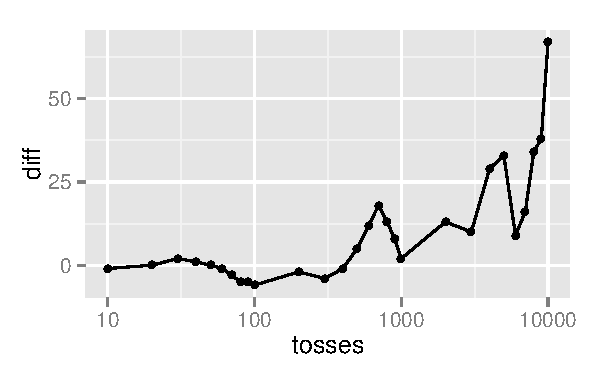
\includegraphics{figures/diff.pdf}
    \caption{Difference from expected}
    \label{fig:diff}
  \end{figure}

  \begin{figure}[H]
    \centering
    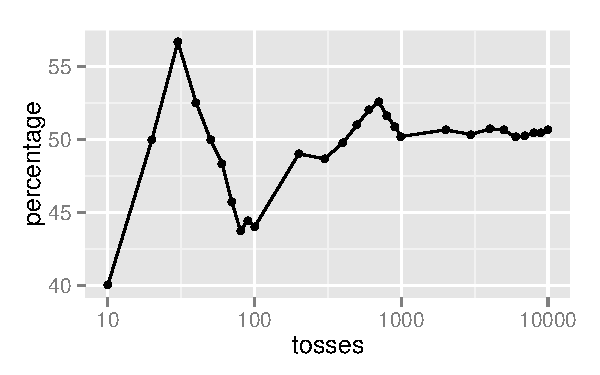
\includegraphics{figures/percentage.pdf}
    \caption{Percentage heads}
    \label{fig:percentage}
  \end{figure}

  \subsection{Notes}
  \begin{itemize*}
    \item as number of tosses in creases, absolute value of difference also
      increases
    \item difference increases more slowly than number of tosses, so percentage
      difference decreases
    \item over time difference might eventually go to a large negative number
  \end{itemize*}

  \subsection{Exercises}

  \begin{enumerate}
    \item Which is the better bet: 10 tosses or 100 tosses?
      \begin{enumerate*}
        \item win if more than 60\% heads
        \item win if more than 40\% heads
        \item win if between 40\% and 60\% heads
        \item win if exactly 50\% heads 
      \end{enumerate*}
  \end{enumerate}

  \section{Expected Value and Standard Error}
  \subsection{Expected Value}
  If head is worth 1 and tails 0, what is the expected value for 100 flips?

  \begin{itemize*}
    \item $\mu = 0.5$; $0.5 \cdot 100 = 50$
    \item $50 \pm SE$
  \end{itemize*}

  \subsection{Standard Error}
  \[
    SE = \sigma \cdot \sqrt{n}
  \]

  \begin{itemize*}
    \item larger SD leads to larger SE
    \item larger number of samples leads to larger SE. you expect a larger
      absolute deviation from the mean after 1000 samples than after 100
      samples.
    \item SE is just like SD. observed values are usually within 2 SEs of $\mu$.
      same rules as SD (68\%, 97\%, etc.)
  \end{itemize*}

  \subsection{Box Model}
  A good model for many problems is drawing tickets from a box.
  \begin{itemize*}
    \item each ticket labeled with the value
    \item more tickets for more likely outcomes
    \item compute $\mu$ and $\sigma$ for the tickets
  \end{itemize*}

  A shortcut for finding SD when there are only two kinds of tickets is:
  \[
    (min - max) \cdot \sqrt{proportion_{min} \cdot proportion_{max}}
  \]

  \subsection{Examples}
  \begin{enumerate}
    \item 100 Micholob drinkers tried Schlitz live at half time of super bowl in
      a live taste test (actual Super Bowl commercial from the 80s). 
      
      Assuming the two beers are indistinguishable, what's the chance that at
      least 40 of the Micholob drinkers will prefer Schlitz?

      \begin{solution}
        If nobody can tell the difference, the expected value is 50.

        The standard error is:
        \[
          EV = 10 \sqrt 0.5 = 5
        \]

        The chance of less than 40 people preferring Schlitz is the chance of
        being more than 2 SDs less from the mean, or around 1\%
      \end{solution}

    \item Play roulette 100 times, betting \$1 on 10 to win. Winning bet
      pays \$35. How much should you expect to lose?
      \begin{solution}
        box model: 37 -1 tickets and 1 35 ticket

        \[
          \mu = \frac{35 - 37}{38} = -0.05
        \]

        After 100 plays:
        \[
          100 \cdot -0.05 = -5
        \]

        \begin{align*}
          \sigma & = 36 \cdot \sqrt{\frac{1}{38} \cdot \frac{37}{38}} \\
                 & \approx 5.76 \\
          SE     & \approx \sqrt{100} \cdot 5.76 = 57.6 \\
        \end{align*}

        He should expect to lose:
        \[
          -5 \pm 57.6
        \]

        The large SE is what keeps people playing.

      \end{solution}

    \item Play roulette 100 times, with section bet with 2 to 1 payoff and 12
      chances in 38 to win

      \begin{solution}
        \paragraph{section bet}
        box model: 26 -\$1 tickets and 12 \$2 ticket

        \[
          \mu = \frac{24 - 26}{38} \approx -0.05
        \]

        After 100 plays:
        \[
          100 \cdot -0.05 = -\$5
        \]

        \begin{align*}
          \sigma &= 3 \cdot \sqrt{\frac{12}{38} \cdot \frac{26}{38}} \\
          & \approx 1.39 \\
          \\
          SE &\approx \sqrt{100} \cdot 1.39 = 13.9 \\
        \end{align*}

        He should expect to lose:
        \[
          -5 \pm 13.9
        \]

      \end{solution}
    \item Play roulette 100 times, with red bet with even payoff and 18
      chances in 38 to win

      \begin{solution}
        box model: 20 -\$1 tickets and 18 \$1 ticket

        \[
          \mu = \frac{18 - 20}{38} \approx -0.05
        \]

        After 100 plays:
        \[
          100 \cdot -0.05 = -\$5
        \]

        \begin{align*}
          \sigma & = 2 \cdot \sqrt{\frac{18}{38} \cdot \frac{20}{38}} \\
                 & \approx 1 \\
          \\
          SE     & \approx \sqrt{100} \cdot 1 = 10 \\
        \end{align*}

        He should expect to lose:
        \[
          -5 \pm 10
        \]
      \end{solution}

    \item In a week there are 25,000 independent \$1 plays on red in a casino.
      What is the chance the casino will win more than \$1000 on these plays?

      \begin{solution}
        \begin{align*}
          \mu & = 0.05 \cdot 25,000 = 1250
          SE  & \approx \sqrt{25000} \cdot 1 = \$158 \\
        \end{align*}

        Convert \$1000 to standard units:
        \[
          \frac{1000 - 1250}{158} \approx -1.58 \\
        \]

        Use table A, there is about a 95\% chance of making at least \$1000.

        If you do a similar calculation with gradually increasing bet sizes and
        fewer bets, you find:

        \begin{table}[H]
        \centering
          \begin{tabular}{rrrrrrr}
            \toprule
               & n        & amount   & sd       & se       & z     & p \\
            \midrule
            1  & 25000.00 & 1.00     & 1.00     & 157.89   & -1.58 & 0.94 \\
            2  & 1000.00  & 25.00    & 24.97    & 789.47   & -0.32 & 0.62 \\
            3  & 100.00   & 250.00   & 249.65   & 2496.53  & -0.10 & 0.54 \\
            4  & 10.00    & 2500.00  & 2496.53  & 7894.74  & -0.03 & 0.51 \\
            5  & 1.00     & 25000.00 & 24965.35 & 24965.35 & -0.01 & 0.50 \\
            \bottomrule
          \end{tabular}
        \end{table}

        For a single bet the casino has a 20/38 (53\%) chance of making \$25,000
        and a 18/38 (47\%) chance of losing \$25,000.

        Since the casino is a business, it is probably happier with more small
        bets so it can be more confident of making money.

        Of course as SE increases, the chance of the casino making a lot of
        money on a single bet also increases.
        
      \end{solution}

    \item What happens to a gambler that bets \$1 on each number, including 0
      and 00? A winning bet on a single number pays \$35.

      \begin{solution}
        He'll definitely win \$35 but lose \$37 on all the other numbers, for a
        net loss of \$2. The casino likes it when you spread your bets.
      \end{solution}

    \item Tickets are drawn at random with replacement from a box of numbered
      tickets. The sum of 25 draws has expected value equal to 50 with SE of 10.
      Find the expected value and SE for 100 draws.

      \begin{solution}
        Since $\mu = 2$, the expected value is 200.

        \begin{align*}
          5 \cdot SD & = 10 \\
          SD   & = 2 \\
          \\
          SE   & = 10 \cdot SD \\
               & = 20 \\
        \end{align*}
        
      \end{solution}

    \item A box contains 10 tickets. Each ticket is marked with a number between
      -5 and 5. The numbers are not all the same but their average is 0. There
      are two choices:
      \begin{itemize*}
        \item 100 draws and you win if the sum is between -15 and 15
        \item 200 draws and you win if the sum is between -30 and 30
      \end{itemize*}

      Which choice gives you a better chance of winning?

      \begin{solution}
        The second choice is better.  Doubling the number of draws only
        increases the SE by a factor of

        $\sqrt{2} \approx 1.4$. 

%         For example, suppose the tickets are all either -5 or 5.

%         For 100 draws:
%         \begin{align*}
%           SD & = 10 \sqrt{\frac{1}{2} \cdot \frac{1}{2}} \\
%              & = 5 \\
%           \\
%           SE & = 10 \cdot 5
%              & = 50 \\
%           \\
%           z_{15} & = \frac{15}{50} \\
%                  & = 0.3 \\
%         \end{align*}

%         For 200 draws, SD is the same:
%         \begin{align*}
%           SE & = \sqrt{200} \cdot 5
%              & \approx 71 \\
%           \\
%           z_{30} & = \frac{30}{71} \\
%                  & = 0.42 \\
%         \end{align*}

        Suppose the SD of the numbers was 1.5.
        
        The SE for the first choice would $\sqrt{100} \cdot 1.5 = 15$. You would
        have a 68\% chance of winning since you are betting on the result being
        within one SD of the mean. 
        
        The SE for the second choice would be $\sqrt{200} \cdot 1.5 \approx 21$.
        You would have a larger than 68\% chance of winning since 30 is more
        than one SE away from the mean.

      \end{solution}
  \end{enumerate}

  \section{Sampling Distribution}

  Standard error is total error to expect (Figure \ref{fig:diff}), which goes up
  as the number of trials increases.

  Estimate of $\mu$ (Figure \ref{fig:percentage}), gets closer
  as the number of trials increases.

  \begin{align*}
    x            & = n \mu + SE \\
    \bar{x}      & = \mu + \frac{SE}{n} \\
                 & = \mu + \frac{\sigma \sqrt{n}}{n} \\
                 & = \mu + \frac{\sigma}{\sqrt{n}} \\
    \\
    sd_{\bar{x}} & = \frac{\sigma}{\sqrt{n}} \\
  \end{align*}

  \begin{itemize*}
    \item $\frac{\sigma}{\sqrt{n}}$ is how far $\bar{x}$ is likely to differ
      from $\mu$.
    \item like SD: 68\% of the time $\bar{x}$ is within this distance of
      $\mu$.
  \end{itemize*}

  Example of 100 coin tosses:
  \begin{align*}
    \sigma        & = \frac{1}{2} \\
    \mu           & = \frac{1}{2} \\
    SE            & = 10 \cdot 0.5 \\
                  & = 5 \\
     sd_{\bar{x}} & = \frac{5}{\sqrt{100}} \\
                  & = 0.5 \\
  \end{align*}

  \section{Central Limit Theorem}
  \subsection{Notes}

  For a reasonable sized sample, the distribution of $\bar{x}$ is $N(\mu,
  \frac{\sigma}{\sqrt{n}})$

  \begin{itemize*}
    \item average of sample is representative of average of population
    \item Doesn't matter if population distribution is normal (coin flipping
      isn't Normal, for example)
    \item SD of sampling distribution always smaller than SD of population
      distribution.
    \item sampling distribution often more normal than population distribution

    \item sampling distribution won't, in general, look anything like population
      distribution.
  \end{itemize*}

  The population size doesn't matter---only sample size matters. For example, if
  you were trying to find the average weight of people in TX vs people in WA,
  you would be just as accurate in either case with a sample of 500. The number
  of people in the population doesn't appear in the formula.

  Use example of buses full of:
  \begin{itemize*}
    \item marathon runners
    \item ``Overeaters Anonymous'' convention participants
  \end{itemize*}

  There is some overlap between the populations because there are some heavy
  marathoners and some light (short, long-term dieters, etc.) overeaters. But
  you could examine the average for a bus full of people and tell whether the
  bus contains a sample of marathoners or a sample of overeaters.

  \subsection{Examples}
  \begin{enumerate}

    \item You want to do a poll to find out how many people have seen the latest
      episode of ``Walking Dead'' with an accuracy of $\pm 1\%$. How big should
      the sample be? 

      \begin{solution}
        The largest the standard deviation might be is (min = 0, max = 1):
        \[
          \sigma = \sqrt{\frac{1}{2} \cdot \frac{1}{2}} = 0.5
        \]

        Assuming the worst case:
        \begin{align*}
          sd_{\bar{x}} & = \frac{\sigma}{\sqrt{n}} \\
          n            & = \left( \frac{\sigma}{sd_{\bar{x}}} \right)^2 \\
          n            & = \left( \frac{0.5}{0.01} \right)^2 \\
                       & = 2500 \\
        \end{align*}

        With a sample of 2500 people, you will be within 1\% of the actual value
        68\% of the time, even if half the people have seen the show. 
        
        If you need a higher than 68\% confidence, you could take a larger
        sample.

        If more or less than half have seen the show, the survey will be even
        more accurate, since this will make the standard deviation smaller than
        0.5 (see below, if time permits).

        If you take the sample and find that only about 10\% of the population
        has seen the show, you can be even more confident in your estimate:

        \begin{align*}
          \sigma & = \sqrt{\frac{1}{10} \cdot \frac{9}{10}} = 0.3 \\
          \\
          sd_{\bar{x}} & = \frac{0.3}{\sqrt{2500}} = 0.006 \\
        \end{align*}

        With the new standard deviation of 0.006, 1\% is now 1.6 SDs from the
        mean: 
        
        \begin{align*}
          0.01 & = x \cdot 0.006 \\
          x   & \approx 1.6 \\
        \end{align*}
        From Table A, the probability of being more than 1.6 SDs from the mean
        is only 10\%.

      \end{solution}

    \item You observe 1000 spins of a roulette wheel and find that 550 came out
      red. What's the probability of this if the wheel is fair?

      \begin{solution}
        Find the standard deviation for the sample distribution:
        \begin{align*}
          \sigma & = \sqrt{\frac{18}{38} \cdot \frac{20}{38}} \approx 0.5 \\
          \\
          sd_{\bar{x}} & = \frac{0.5}{\sqrt{1000}} \approx 0.016 \\
        \end{align*}

        Convert the observed mean to a z-score:
        \begin{align*}
          p        & = \frac{550}{1000} = 0.55 \\
          \\
          z_{0.55} & = \frac{0.55 - 0.5}{0.016} = 3.125 \\
        \end{align*}

        The value is more than three standard deviations away from the mean. The
        chance of this happening by chance is slim.

        68\% of the time, the percentage of red would be between 0.484 and
        0.516. Converted back to rolls, you would expect that 68\% of the time
        you would see between 484 and 516 reds in 1000 spins.

      \end{solution}
  \end{enumerate}
\end{document}

